\documentclass[12pt,a4paper]{article}
\usepackage[utf8]{inputenc}
\usepackage[francais]{babel}
\usepackage[T1]{fontenc}
\usepackage{amsmath}
\usepackage{amsfonts}
\usepackage{amssymb}
\usepackage{graphicx}
\usepackage{kpfonts}

\usepackage{siunitx}

\author{Mathieu Leocmach}
\begin{document}

\begin{figure}
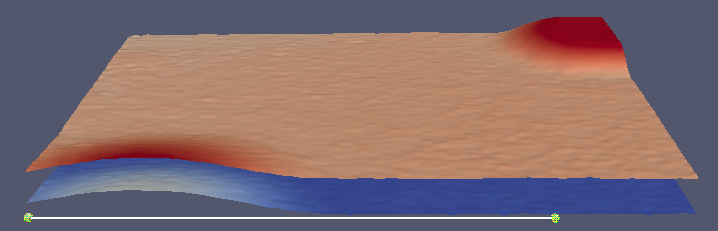
\includegraphics[width=\textwidth]{plots_0117.png}
\caption{Un exemple de cloque en train de croitre (premier plan). Au fond : une cloque qui a touché une paroi. La barre fait \SI{1}{\milli\metre}.}
\end{figure}

On considère une cloque de diamètre $\lambda$ dont le contour touche la paroi inférieure et dont le sommet s'est élevé d'une hauteur $A(t)$ à l'instant $t$. On considère que $A \ll \lambda$, donc l'aire reste $\lambda^2$.

En généralisant Vella PRL 2009, on considère $\sigma$ une contrainte s'exerçant uniformément sur la cloque suivant $z$. Minimiser l'énargie revient à minimiser la fonctionnelle
\begin{equation}
\mathcal{F} = \int_0^{\lambda/2}\left\lbrace\frac{1}{2} B \theta_s^2 + \sigma z - \Sigma \left[1-\frac{\Delta \lambda}{\lambda} - \cos\theta\right] \right\rbrace ds
\end{equation}
avec $s$ l'abcisse curviligne, $\theta(s)$ l'angle avec l'horizontale, $B$ le module de flexion $B \sim E h^3 /12 / (1-\nu^2) \sim G' h^3/10$.

Une longueur caractéristique apparaît :
\begin{equation}
\lambda^* = \left(\frac{B}{\sigma}\right)^\frac{1}{3}
\end{equation}
au dessus de laquelle $\sigma$ est capable d'écraser la cloque.

\paragraph*{Si $\sigma = \Delta\rho g h$}, c'est une longueur élastogravitaire

Dans notre cas $\Delta\rho\simeq 10\%w = \SI{100}{\kilo\gram\per\metre^3}$, d'où
\begin{equation}
\lambda^* \sim \left(\frac{\num{6e-12}}{100\times 10 \num{50e-6}}\right)^\frac{1}{3} \sim \SI{5}{\centi\metre}
\end{equation}
Donc la gravité n'influe pas, ce qui est confirmé par un échantillon vertical plissant.

\paragraph*{Si $\sigma$ est une pression de Darcy $P$} telle que 
\begin{equation}
\vec{v} = - \frac{l_p^2}{\eta}  \vec{\nabla} P
\label{eq:Darcy}
\end{equation}
avec $v$ le flux volumique à travers la surface, c'est-à-dire la vitesse de déplacement du film, $l_p$ la taille des pores, $\eta$ la viscosité du solvant et $\vec{\nabla} P \sim -P/h$. Alors,
\begin{equation}
\lambda^* \sim \left(\frac{B l_p^2}{\eta v h}\right)^\frac{1}{3}
\end{equation}

On a mesuré $v\simeq \SI{0.2}{\micro\metre\per\second}$, ce qui donne 
\begin{equation}
\lambda^* \sim \left(\frac{\num{6e-12} (\num{4e-6})^2}{10^{-3} \times \num{0.2e-6} \times \num{50e-6}}\right)^\frac{1}{3} \simeq \SI{2}{\milli\metre}
\end{equation}

Il manque une équation qui nous permettrait d'obtenir $v$ ou $\lambda$ à partir des données du problème.

\pagebreak

La courbure $\kappa$ est de l'ordre de $A/\lambda^2$ et l'énergie de courbure est
\begin{equation}
U_B \sim B  \kappa^2  \lambda^2 \sim B  \left(\frac{A}{\lambda}\right)^2
\end{equation}
avec $B$ le module de flexion $B \sim E h^3 /12 / (1-\nu^2) \sim G' h^3/10$

La déflexion du film crée une différence de pression $P$ entre le dessous et le dessus. Le travail associé est $W \sim P  A  \lambda^2$

Si on égale $U_B$ et $W$ (je dois faire une hypothèse quand je fais ça, mais je n'arrive pas à mettre le doigt dessus), on trouve $P \sim BA/\lambda^4$

Une autre équation vient de la loi de Darcy qui donne le débit volumique $v$ à travers un poreux 
\begin{equation}
\vec{v} = - \frac{l_p^2}{\eta}  \vec{\nabla} P
\label{eq:Darcy}
\end{equation}
avec $l_p$ la taille des pores, $\eta$ la viscosité du solvant et $\vec{\nabla} P \sim -P/h$.

Le volume sous le film est $V \sim A \lambda^2$ et sa dérivée temporelle est
\begin{equation}
\frac{dV}{dt} \sim \lambda^2  \frac{dA}{dt}
\label{eq:var_vol}
\end{equation}
qui s'exprime aussi en fonction du débit à travers la surface
\begin{equation}
\frac{dV}{dt} \sim \lambda^2  v
\label{eq:debit}
\end{equation}

En utilisant les équations (\ref{eq:Darcy}), (\ref{eq:var_vol}) et (\ref{eq:debit}), on obtient
\begin{equation}
\frac{dA}{dt} \sim v \sim \frac{l_p^2  P}{eta * h}
\end{equation}

Et en réutilisant l'expression de la pression ci-dessus, on trouve
\begin{equation}
\frac{dA}{dt} \sim \frac{A}{\tau}
\end{equation}
donc une croissance exponentielle de temps caractéristique
\begin{equation}
\tau = \frac{\eta h  \lambda^4} {B l_p^2}
\end{equation}

Application numérique :
\begin{align}
\lambda \sim & \SI{1}{\milli\metre}\\
h \sim & \SI{50}{\micro\metre}\\
G^\prime \sim & \SI{500}{\pascal}\\
B \sim & 50 \times (50\cdot 10^{-6})^3 \sim \SI{6e-12}{\joule}\\
\tau \sim & \frac{10^{-3} \times 50\cdot 10^{-6} \times (10^{-3})^4}{6 \cdot 10^{-12} \times (4 \cdot 10^{-6})^{-2}} \sim \SI{500}{\second}
\end{align}

\end{document}